% Options for packages loaded elsewhere
\PassOptionsToPackage{unicode}{hyperref}
\PassOptionsToPackage{hyphens}{url}
%
\documentclass[
]{article}
\usepackage{amsmath,amssymb}
\usepackage{lmodern}
\usepackage{ifxetex,ifluatex}
\ifnum 0\ifxetex 1\fi\ifluatex 1\fi=0 % if pdftex
  \usepackage[T1]{fontenc}
  \usepackage[utf8]{inputenc}
  \usepackage{textcomp} % provide euro and other symbols
\else % if luatex or xetex
  \usepackage{unicode-math}
  \defaultfontfeatures{Scale=MatchLowercase}
  \defaultfontfeatures[\rmfamily]{Ligatures=TeX,Scale=1}
\fi
% Use upquote if available, for straight quotes in verbatim environments
\IfFileExists{upquote.sty}{\usepackage{upquote}}{}
\IfFileExists{microtype.sty}{% use microtype if available
  \usepackage[]{microtype}
  \UseMicrotypeSet[protrusion]{basicmath} % disable protrusion for tt fonts
}{}
\makeatletter
\@ifundefined{KOMAClassName}{% if non-KOMA class
  \IfFileExists{parskip.sty}{%
    \usepackage{parskip}
  }{% else
    \setlength{\parindent}{0pt}
    \setlength{\parskip}{6pt plus 2pt minus 1pt}}
}{% if KOMA class
  \KOMAoptions{parskip=half}}
\makeatother
\usepackage{xcolor}
\IfFileExists{xurl.sty}{\usepackage{xurl}}{} % add URL line breaks if available
\IfFileExists{bookmark.sty}{\usepackage{bookmark}}{\usepackage{hyperref}}
\hypersetup{
  pdftitle={Statistical Learning Project},
  pdfauthor={Filippo Santin, Gurjeet Singh, Francesca Zen},
  hidelinks,
  pdfcreator={LaTeX via pandoc}}
\urlstyle{same} % disable monospaced font for URLs
\usepackage[margin=1in]{geometry}
\usepackage{color}
\usepackage{fancyvrb}
\newcommand{\VerbBar}{|}
\newcommand{\VERB}{\Verb[commandchars=\\\{\}]}
\DefineVerbatimEnvironment{Highlighting}{Verbatim}{commandchars=\\\{\}}
% Add ',fontsize=\small' for more characters per line
\usepackage{framed}
\definecolor{shadecolor}{RGB}{248,248,248}
\newenvironment{Shaded}{\begin{snugshade}}{\end{snugshade}}
\newcommand{\AlertTok}[1]{\textcolor[rgb]{0.94,0.16,0.16}{#1}}
\newcommand{\AnnotationTok}[1]{\textcolor[rgb]{0.56,0.35,0.01}{\textbf{\textit{#1}}}}
\newcommand{\AttributeTok}[1]{\textcolor[rgb]{0.77,0.63,0.00}{#1}}
\newcommand{\BaseNTok}[1]{\textcolor[rgb]{0.00,0.00,0.81}{#1}}
\newcommand{\BuiltInTok}[1]{#1}
\newcommand{\CharTok}[1]{\textcolor[rgb]{0.31,0.60,0.02}{#1}}
\newcommand{\CommentTok}[1]{\textcolor[rgb]{0.56,0.35,0.01}{\textit{#1}}}
\newcommand{\CommentVarTok}[1]{\textcolor[rgb]{0.56,0.35,0.01}{\textbf{\textit{#1}}}}
\newcommand{\ConstantTok}[1]{\textcolor[rgb]{0.00,0.00,0.00}{#1}}
\newcommand{\ControlFlowTok}[1]{\textcolor[rgb]{0.13,0.29,0.53}{\textbf{#1}}}
\newcommand{\DataTypeTok}[1]{\textcolor[rgb]{0.13,0.29,0.53}{#1}}
\newcommand{\DecValTok}[1]{\textcolor[rgb]{0.00,0.00,0.81}{#1}}
\newcommand{\DocumentationTok}[1]{\textcolor[rgb]{0.56,0.35,0.01}{\textbf{\textit{#1}}}}
\newcommand{\ErrorTok}[1]{\textcolor[rgb]{0.64,0.00,0.00}{\textbf{#1}}}
\newcommand{\ExtensionTok}[1]{#1}
\newcommand{\FloatTok}[1]{\textcolor[rgb]{0.00,0.00,0.81}{#1}}
\newcommand{\FunctionTok}[1]{\textcolor[rgb]{0.00,0.00,0.00}{#1}}
\newcommand{\ImportTok}[1]{#1}
\newcommand{\InformationTok}[1]{\textcolor[rgb]{0.56,0.35,0.01}{\textbf{\textit{#1}}}}
\newcommand{\KeywordTok}[1]{\textcolor[rgb]{0.13,0.29,0.53}{\textbf{#1}}}
\newcommand{\NormalTok}[1]{#1}
\newcommand{\OperatorTok}[1]{\textcolor[rgb]{0.81,0.36,0.00}{\textbf{#1}}}
\newcommand{\OtherTok}[1]{\textcolor[rgb]{0.56,0.35,0.01}{#1}}
\newcommand{\PreprocessorTok}[1]{\textcolor[rgb]{0.56,0.35,0.01}{\textit{#1}}}
\newcommand{\RegionMarkerTok}[1]{#1}
\newcommand{\SpecialCharTok}[1]{\textcolor[rgb]{0.00,0.00,0.00}{#1}}
\newcommand{\SpecialStringTok}[1]{\textcolor[rgb]{0.31,0.60,0.02}{#1}}
\newcommand{\StringTok}[1]{\textcolor[rgb]{0.31,0.60,0.02}{#1}}
\newcommand{\VariableTok}[1]{\textcolor[rgb]{0.00,0.00,0.00}{#1}}
\newcommand{\VerbatimStringTok}[1]{\textcolor[rgb]{0.31,0.60,0.02}{#1}}
\newcommand{\WarningTok}[1]{\textcolor[rgb]{0.56,0.35,0.01}{\textbf{\textit{#1}}}}
\usepackage{longtable,booktabs,array}
\usepackage{calc} % for calculating minipage widths
% Correct order of tables after \paragraph or \subparagraph
\usepackage{etoolbox}
\makeatletter
\patchcmd\longtable{\par}{\if@noskipsec\mbox{}\fi\par}{}{}
\makeatother
% Allow footnotes in longtable head/foot
\IfFileExists{footnotehyper.sty}{\usepackage{footnotehyper}}{\usepackage{footnote}}
\makesavenoteenv{longtable}
\usepackage{graphicx}
\makeatletter
\def\maxwidth{\ifdim\Gin@nat@width>\linewidth\linewidth\else\Gin@nat@width\fi}
\def\maxheight{\ifdim\Gin@nat@height>\textheight\textheight\else\Gin@nat@height\fi}
\makeatother
% Scale images if necessary, so that they will not overflow the page
% margins by default, and it is still possible to overwrite the defaults
% using explicit options in \includegraphics[width, height, ...]{}
\setkeys{Gin}{width=\maxwidth,height=\maxheight,keepaspectratio}
% Set default figure placement to htbp
\makeatletter
\def\fps@figure{htbp}
\makeatother
\setlength{\emergencystretch}{3em} % prevent overfull lines
\providecommand{\tightlist}{%
  \setlength{\itemsep}{0pt}\setlength{\parskip}{0pt}}
\setcounter{secnumdepth}{-\maxdimen} % remove section numbering
\ifluatex
  \usepackage{selnolig}  % disable illegal ligatures
\fi

\title{Statistical Learning Project}
\author{Filippo Santin, Gurjeet Singh, Francesca Zen}
\date{18/5/2021}

\begin{document}
\maketitle

\hypertarget{introduction}{%
\section{1 Introduction}\label{introduction}}

In the following report we present an analysis computed on stroke
disease, and we try to explain from statistical analysis some
correlation factors and statistics of the given features/predictors by
constructing predictive models in order to assess possible linear and
non-linear relationships of features (predictors) to predict a stroke
disease in a person (predicted variable).

``Stroke'' is the medical term for damage to brain tissue or the death
of a portion of it, due to insufficient blood supply to an area of the
brain.

Our aim is to see if and how the variables we are dealing with are
related, in order to predict which individual is more probable to have a
stroke.

The symptoms of stroke vary from patient to patient, depending on the
severity of the condition, the affected brain area, causes, type of
stroke, etc.

Stroke is characterized by sudden onset and for this reason it involves
the need for immediate therapeutic intervention and adapted to the needs
of the patient. In this sense, looking for relation between features may
help to prevent or assess it.

In order to have a guide for the interpretation of the data we underline
the following information:

\begin{itemize}
\tightlist
\item
  The normal values of glucose level are between 60 and 110 mg/dl and
  with a value greater than 126 mg/dl a person is considered diabetic;
\item
  a body mass index (BMI) between 18.5-24.9 indicates a normal/healthy
  weight, below 18.5 indicates underweight, 25.0-29.9 indicates
  overweight and above 30.0 indicates obese person.
\end{itemize}

\hypertarget{exploring-the-dataset}{%
\section{2 Exploring the Dataset}\label{exploring-the-dataset}}

The dataset we used is provided by Kaggle \footnote{\url{https://www.kaggle.com/fedesoriano/stroke-prediction-dataset}}
and it is composed of 5,110 entries with a total of 12 columns:
\texttt{id}, \texttt{gender}, \texttt{age}, \texttt{hypertension},
\texttt{heart\_disease}, \texttt{ever\_married}, \texttt{work\_type},
\texttt{Residence\_type}, \texttt{avg\_glucose\_level}, \texttt{bmi},
\texttt{smoking\_status}, \texttt{stroke}.

\begin{Shaded}
\begin{Highlighting}[]
\FunctionTok{library}\NormalTok{(knitr)}
\NormalTok{stroke\_data }\OtherTok{\textless{}{-}} \FunctionTok{read.csv}\NormalTok{(}\StringTok{\textquotesingle{}healthcare{-}dataset{-}stroke{-}data.csv\textquotesingle{}}\NormalTok{)}
\FunctionTok{kable}\NormalTok{(stroke\_data[}\DecValTok{1}\SpecialCharTok{:}\DecValTok{5}\NormalTok{,], }\AttributeTok{format =} \StringTok{\textquotesingle{}simple\textquotesingle{}}\NormalTok{, }\AttributeTok{align=}\StringTok{\textquotesingle{}ccccccccc\textquotesingle{}}\NormalTok{, }
      \AttributeTok{col.names =} \FunctionTok{c}\NormalTok{(}\StringTok{\textquotesingle{}id\textquotesingle{}}\NormalTok{,}\StringTok{\textquotesingle{}gender\textquotesingle{}}\NormalTok{,}\StringTok{\textquotesingle{}age\textquotesingle{}}\NormalTok{, }\StringTok{\textquotesingle{}hypert.\textquotesingle{}}\NormalTok{, }\StringTok{\textquotesingle{}hd\textquotesingle{}}\NormalTok{ ,}\StringTok{\textquotesingle{}ev\_marr\textquotesingle{}}\NormalTok{,}
                    \StringTok{\textquotesingle{}work\_type\textquotesingle{}}\NormalTok{,}\StringTok{\textquotesingle{}res\_type\textquotesingle{}}\NormalTok{,}\StringTok{\textquotesingle{}glucose\textquotesingle{}}\NormalTok{, }\StringTok{\textquotesingle{}bmi\textquotesingle{}}\NormalTok{,}\StringTok{\textquotesingle{}smoking\textquotesingle{}}\NormalTok{,}\StringTok{\textquotesingle{}stroke\textquotesingle{}}\NormalTok{))}
\end{Highlighting}
\end{Shaded}

\begin{longtable}[]{@{}cccccccccccc@{}}
\toprule
id & gender & age & hypert. & hd & ev\_marr & work\_type & res\_type &
glucose & bmi & smoking & stroke \\
\midrule
\endhead
9046 & Male & 67 & 0 & 1 & Yes & Private & Urban & 228.69 & 36.6 &
formerly smoked & 1 \\
51676 & Female & 61 & 0 & 0 & Yes & Self-employed & Rural & 202.21 & N/A
& never smoked & 1 \\
31112 & Male & 80 & 0 & 1 & Yes & Private & Rural & 105.92 & 32.5 &
never smoked & 1 \\
60182 & Female & 49 & 0 & 0 & Yes & Private & Urban & 171.23 & 34.4 &
smokes & 1 \\
1665 & Female & 79 & 1 & 0 & Yes & Self-employed & Rural & 174.12 & 24 &
never smoked & 1 \\
\bottomrule
\end{longtable}

\hypertarget{preprocessing}{%
\subsection{2.1 Preprocessing}\label{preprocessing}}

The preliminary part of the analysis focuses on the study of the dataset
and its pre-processing: we looked at the \texttt{id} column and verified
that all the data collected was referring to different people, thus no
recidivist status were involved. After this check we removed the column
from the dataset as it does not hold useful information for our study.

\begin{Shaded}
\begin{Highlighting}[]
\NormalTok{stroke\_data}\OtherTok{\textless{}{-}}\NormalTok{stroke\_data[,}\SpecialCharTok{{-}}\DecValTok{1}\NormalTok{]}
\end{Highlighting}
\end{Shaded}

In order to use the variables through the analysis we transformed the
categorical variables into factors:

\begin{Shaded}
\begin{Highlighting}[]
\NormalTok{stroke\_data}\SpecialCharTok{$}\NormalTok{gender}\OtherTok{\textless{}{-}} \FunctionTok{as.factor}\NormalTok{(stroke\_data}\SpecialCharTok{$}\NormalTok{gender)}
\NormalTok{stroke\_data}\SpecialCharTok{$}\NormalTok{ever\_married}\OtherTok{\textless{}{-}}\FunctionTok{as.factor}\NormalTok{(stroke\_data}\SpecialCharTok{$}\NormalTok{ever\_married)}
\NormalTok{stroke\_data}\SpecialCharTok{$}\NormalTok{work\_type}\OtherTok{\textless{}{-}}\FunctionTok{as.factor}\NormalTok{(stroke\_data}\SpecialCharTok{$}\NormalTok{work\_type)}
\NormalTok{stroke\_data}\SpecialCharTok{$}\NormalTok{Residence\_type}\OtherTok{\textless{}{-}}\FunctionTok{as.factor}\NormalTok{(stroke\_data}\SpecialCharTok{$}\NormalTok{Residence\_type)}
\NormalTok{stroke\_data}\SpecialCharTok{$}\NormalTok{smoking\_status}\OtherTok{\textless{}{-}}\FunctionTok{as.factor}\NormalTok{(stroke\_data}\SpecialCharTok{$}\NormalTok{smoking\_status)}
\end{Highlighting}
\end{Shaded}

In addition, the variable \texttt{bmi} was not numeric because of the
presence of ``N/A'' string values which identify missing information,
hence we transformed it into numeric values and then removed the NA
values generated.

\begin{Shaded}
\begin{Highlighting}[]
\NormalTok{stroke\_data}\SpecialCharTok{$}\NormalTok{bmi }\OtherTok{\textless{}{-}} \FunctionTok{as.numeric}\NormalTok{(stroke\_data}\SpecialCharTok{$}\NormalTok{bmi)}
\end{Highlighting}
\end{Shaded}

\begin{verbatim}
## Warning: NA introdotti per coercizione
\end{verbatim}

\begin{Shaded}
\begin{Highlighting}[]
\NormalTok{stroke\_data}\OtherTok{\textless{}{-}} \FunctionTok{na.omit}\NormalTok{(stroke\_data)}
\end{Highlighting}
\end{Shaded}

We ended up having 4,909 entries and 11 total columns. Here we give a
quick overview of the main information about the dataset:

\begin{Shaded}
\begin{Highlighting}[]
\FunctionTok{summary}\NormalTok{(stroke\_data)}
\end{Highlighting}
\end{Shaded}

\begin{verbatim}
##     gender          age         hypertension     heart_disease    ever_married
##  Female:2897   Min.   : 0.08   Min.   :0.00000   Min.   :0.0000   No :1705    
##  Male  :2011   1st Qu.:25.00   1st Qu.:0.00000   1st Qu.:0.0000   Yes:3204    
##  Other :   1   Median :44.00   Median :0.00000   Median :0.0000               
##                Mean   :42.87   Mean   :0.09187   Mean   :0.0495               
##                3rd Qu.:60.00   3rd Qu.:0.00000   3rd Qu.:0.0000               
##                Max.   :82.00   Max.   :1.00000   Max.   :1.0000               
##          work_type    Residence_type avg_glucose_level      bmi       
##  children     : 671   Rural:2419     Min.   : 55.12    Min.   :10.30  
##  Govt_job     : 630   Urban:2490     1st Qu.: 77.07    1st Qu.:23.50  
##  Never_worked :  22                  Median : 91.68    Median :28.10  
##  Private      :2811                  Mean   :105.31    Mean   :28.89  
##  Self-employed: 775                  3rd Qu.:113.57    3rd Qu.:33.10  
##                                      Max.   :271.74    Max.   :97.60  
##          smoking_status     stroke       
##  formerly smoked: 837   Min.   :0.00000  
##  never smoked   :1852   1st Qu.:0.00000  
##  smokes         : 737   Median :0.00000  
##  Unknown        :1483   Mean   :0.04257  
##                         3rd Qu.:0.00000  
##                         Max.   :1.00000
\end{verbatim}

\hypertarget{descriptive-statistic}{%
\subsection{2.2 Descriptive Statistic}\label{descriptive-statistic}}

\begin{Shaded}
\begin{Highlighting}[]
\FunctionTok{attach}\NormalTok{(stroke\_data)}
\end{Highlighting}
\end{Shaded}

In order to highlight and study better the data, we used some plots to
study their statistics and distribution. A relevant and important
information is provided by the following barplot, in which we see an
unbalance dataset issue: 209 people on a total of 4909 get a stroke,
i.e.~the 4.25 \% of the people.

\begin{Shaded}
\begin{Highlighting}[]
\FunctionTok{table}\NormalTok{(stroke)}\SpecialCharTok{/}\FunctionTok{dim}\NormalTok{(stroke\_data)[}\DecValTok{1}\NormalTok{]}
\end{Highlighting}
\end{Shaded}

\begin{verbatim}
## stroke
##          0          1 
## 0.95742514 0.04257486
\end{verbatim}

\begin{Shaded}
\begin{Highlighting}[]
\FunctionTok{barplot}\NormalTok{(}\FunctionTok{table}\NormalTok{(stroke)}\SpecialCharTok{/}\FunctionTok{dim}\NormalTok{(stroke\_data)[}\DecValTok{1}\NormalTok{],}
        \AttributeTok{xlab=}\StringTok{\textquotesingle{}probability to have a stroke\textquotesingle{}}\NormalTok{,}\AttributeTok{col =} \FunctionTok{c}\NormalTok{(}\StringTok{\textquotesingle{}\#F8766D\textquotesingle{}}\NormalTok{,}\StringTok{\textquotesingle{}\#00BFC4\textquotesingle{}}\NormalTok{))}
\end{Highlighting}
\end{Shaded}

\begin{center}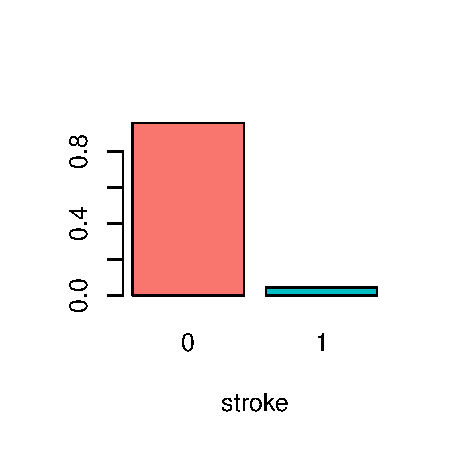
\includegraphics{stat-project-stroke_files/figure-latex/unnamed-chunk-7-1} \end{center}

This value is representative of the real situation in which there are
not many stroke cases compared with the whole population. The incidence
of stroke in Europe at the beginning of the 21st century varies from 95
to 290 cases/100,000\footnote{QUADERNI dell'Italian Journal of Medicine,
  A Journal of Hospital and Internal Medicine, Michele Meschi,volume 8,
  issue 2, March-April 2020}. Furthermore in many clinical diseases
analysis this issue is commonly present.

A visual transformation of the values seen in the \texttt{summary}
function is provided in the following boxplots:

\begin{Shaded}
\begin{Highlighting}[]
\FunctionTok{par}\NormalTok{(}\AttributeTok{mfrow=}\FunctionTok{c}\NormalTok{(}\DecValTok{1}\NormalTok{,}\DecValTok{3}\NormalTok{))}
\FunctionTok{boxplot}\NormalTok{(avg\_glucose\_level, }\AttributeTok{xlab=} \StringTok{\textquotesingle{}average glucose level\textquotesingle{}}\NormalTok{ )}
\FunctionTok{boxplot}\NormalTok{(bmi, }\AttributeTok{xlab =} \StringTok{\textquotesingle{}body mass index\textquotesingle{}}\NormalTok{)}
\FunctionTok{boxplot}\NormalTok{(age, }\AttributeTok{xlab =} \StringTok{\textquotesingle{}age\textquotesingle{}}\NormalTok{,}\AttributeTok{pch=}\DecValTok{20}\NormalTok{)}
\end{Highlighting}
\end{Shaded}

\includegraphics{stat-project-stroke_files/figure-latex/unnamed-chunk-8-1.pdf}

\begin{Shaded}
\begin{Highlighting}[]
\FunctionTok{par}\NormalTok{(}\AttributeTok{mfrow=}\FunctionTok{c}\NormalTok{(}\DecValTok{1}\NormalTok{,}\DecValTok{1}\NormalTok{))}
\end{Highlighting}
\end{Shaded}

From above we can see that in the first two boxplots (starting from the
left) there are lots of outliers, that can also be see from the summary
looking at the difference between the third quantile and the maximum
value in the \texttt{avg\_glucose\_level} and \texttt{bmi} variables.
Actually, they represent real-scenario (few people are affected by high
glucose levels) and possible interesting cases of pathologies bounded
with diabetes. Hence these data points have to be considered during
modeling, they could be helpful to predict stroke cases since as
mentioned in the medical literature stroke could be also due to
complications of diabetes.

In order to compare entities in pairs and judge which of each entity is
preferred, or has a greater amount of some quantitative property we
provide a pair-wise plot. In addition, to involve also the categorical
variables we wrote some useful function:

\begin{Shaded}
\begin{Highlighting}[]
\NormalTok{panel.cor }\OtherTok{\textless{}{-}} \ControlFlowTok{function}\NormalTok{(x, y, }\AttributeTok{digits =} \DecValTok{2}\NormalTok{, }\AttributeTok{prefix =} \StringTok{""}\NormalTok{, cex.cor, ...)\{}
\NormalTok{  usr }\OtherTok{\textless{}{-}} \FunctionTok{par}\NormalTok{(}\StringTok{"usr"}\NormalTok{); }\FunctionTok{on.exit}\NormalTok{(}\FunctionTok{par}\NormalTok{(usr))}
  \FunctionTok{par}\NormalTok{(}\AttributeTok{usr =} \FunctionTok{c}\NormalTok{(}\DecValTok{0}\NormalTok{, }\DecValTok{1}\NormalTok{, }\DecValTok{0}\NormalTok{, }\DecValTok{1}\NormalTok{))}
\NormalTok{  r }\OtherTok{\textless{}{-}} \FunctionTok{abs}\NormalTok{(}\FunctionTok{cor}\NormalTok{(x, y))}
\NormalTok{  txt }\OtherTok{\textless{}{-}} \FunctionTok{format}\NormalTok{(}\FunctionTok{c}\NormalTok{(r, }\FloatTok{0.123456789}\NormalTok{), }\AttributeTok{digits =}\NormalTok{ digits)[}\DecValTok{1}\NormalTok{]}
\NormalTok{  txt }\OtherTok{\textless{}{-}} \FunctionTok{paste0}\NormalTok{(prefix, txt)}
  \ControlFlowTok{if}\NormalTok{(}\FunctionTok{missing}\NormalTok{(cex.cor)) cex.cor }\OtherTok{\textless{}{-}} \FloatTok{0.8}\SpecialCharTok{/}\FunctionTok{strwidth}\NormalTok{(txt)}
  \FunctionTok{text}\NormalTok{(}\FloatTok{0.5}\NormalTok{, }\FloatTok{0.5}\NormalTok{, txt, }\AttributeTok{cex =}\NormalTok{ cex.cor }\SpecialCharTok{*}\NormalTok{ r)}
\NormalTok{\}}

\NormalTok{panel.hist }\OtherTok{\textless{}{-}} \ControlFlowTok{function}\NormalTok{(x, ...)}
\NormalTok{\{}
\NormalTok{  usr }\OtherTok{\textless{}{-}} \FunctionTok{par}\NormalTok{(}\StringTok{"usr"}\NormalTok{); }\FunctionTok{on.exit}\NormalTok{(}\FunctionTok{par}\NormalTok{(usr))}
  \FunctionTok{par}\NormalTok{(}\AttributeTok{usr =} \FunctionTok{c}\NormalTok{(usr[}\DecValTok{1}\SpecialCharTok{:}\DecValTok{2}\NormalTok{], }\DecValTok{0}\NormalTok{, }\FloatTok{1.5}\NormalTok{) )}
\NormalTok{  h }\OtherTok{\textless{}{-}} \FunctionTok{hist}\NormalTok{(x, }\AttributeTok{plot =} \ConstantTok{FALSE}\NormalTok{)}
\NormalTok{  breaks }\OtherTok{\textless{}{-}}\NormalTok{ h}\SpecialCharTok{$}\NormalTok{breaks; nB }\OtherTok{\textless{}{-}} \FunctionTok{length}\NormalTok{(breaks)}
\NormalTok{  y }\OtherTok{\textless{}{-}}\NormalTok{ h}\SpecialCharTok{$}\NormalTok{counts; y }\OtherTok{\textless{}{-}}\NormalTok{ y}\SpecialCharTok{/}\FunctionTok{max}\NormalTok{(y)}
  \FunctionTok{rect}\NormalTok{(breaks[}\SpecialCharTok{{-}}\NormalTok{nB], }\DecValTok{0}\NormalTok{, breaks[}\SpecialCharTok{{-}}\DecValTok{1}\NormalTok{], y, }\AttributeTok{col =} \StringTok{"green"}\NormalTok{, ...)}
\NormalTok{\}}

\NormalTok{box\_plot\_categories }\OtherTok{\textless{}{-}} \ControlFlowTok{function}\NormalTok{(data, y)\{}
\NormalTok{  n\_features }\OtherTok{=} \FunctionTok{length}\NormalTok{(data)}
\NormalTok{  grid }\OtherTok{=} \FunctionTok{round}\NormalTok{(}\FunctionTok{sqrt}\NormalTok{(n\_features))}
  \FunctionTok{print}\NormalTok{(grid)}
  \FunctionTok{par}\NormalTok{(}\AttributeTok{mfrow=}\FunctionTok{c}\NormalTok{(grid, grid))}
\NormalTok{  names }\OtherTok{=} \FunctionTok{colnames}\NormalTok{(data)}
  \ControlFlowTok{for}\NormalTok{ (idx }\ControlFlowTok{in} \FunctionTok{c}\NormalTok{(}\DecValTok{1}\SpecialCharTok{:}\NormalTok{n\_features)) \{}
    \FunctionTok{plot}\NormalTok{(y }\SpecialCharTok{\textasciitilde{}}\NormalTok{ data[, idx], }\AttributeTok{xlab=}\NormalTok{names[idx], }\AttributeTok{main=}\FunctionTok{c}\NormalTok{(}\StringTok{\textquotesingle{}Boxplot y \textasciitilde{} \textquotesingle{}}\NormalTok{, names[idx]))}
\NormalTok{  \}}
  \FunctionTok{par}\NormalTok{(}\AttributeTok{mfrow=}\FunctionTok{c}\NormalTok{(}\DecValTok{1}\NormalTok{, }\DecValTok{1}\NormalTok{))}
\NormalTok{\}}
\end{Highlighting}
\end{Shaded}

And here we show the results from the pairs plot:

\begin{Shaded}
\begin{Highlighting}[]
\FunctionTok{pairs}\NormalTok{(stroke\_data, }\AttributeTok{diag.panel=}\NormalTok{panel.hist, }\AttributeTok{upper.panel=}\NormalTok{panel.cor)}
\end{Highlighting}
\end{Shaded}

\includegraphics{stat-project-stroke_files/figure-latex/unnamed-chunk-10-1.pdf}

The plot shows that the stronger relationships involve quite often the
variable \texttt{age}. There are also other relevant relation between
\texttt{work\_type} and \texttt{ever\_married} plus \texttt{bmi} with
\texttt{working\_status}. In addition, we can see strong collinearity
among th dummy variables \texttt{age}, \texttt{work\_type}, and
\texttt{ever\_married}, so they do not contribute in the fitting.

We go on looking at some intuitive relation of \texttt{stroke} with
\texttt{age},\texttt{bmi} and \texttt{avg\_glucose\_level}:

\begin{Shaded}
\begin{Highlighting}[]
\FunctionTok{par}\NormalTok{(}\AttributeTok{mfrow=}\FunctionTok{c}\NormalTok{(}\DecValTok{1}\NormalTok{,}\DecValTok{3}\NormalTok{))}
\FunctionTok{boxplot}\NormalTok{(avg\_glucose\_level}\SpecialCharTok{\textasciitilde{}}\NormalTok{stroke, }\AttributeTok{xlab=} \StringTok{\textquotesingle{}stroke\textquotesingle{}}\NormalTok{, }
        \AttributeTok{ylab =} \StringTok{\textquotesingle{}average glucose level\textquotesingle{}}\NormalTok{, }\AttributeTok{col =} \FunctionTok{c}\NormalTok{(}\StringTok{\textquotesingle{}\#F8766D\textquotesingle{}}\NormalTok{,}\StringTok{\textquotesingle{}\#00BFC4\textquotesingle{}}\NormalTok{))}
\FunctionTok{boxplot}\NormalTok{(bmi}\SpecialCharTok{\textasciitilde{}}\NormalTok{stroke, }\AttributeTok{xlab =} \StringTok{\textquotesingle{}stroke\textquotesingle{}}\NormalTok{, }\AttributeTok{ylab =} \StringTok{\textquotesingle{}bmi\textquotesingle{}}\NormalTok{,}\AttributeTok{col =} \FunctionTok{c}\NormalTok{(}\StringTok{\textquotesingle{}\#F8766D\textquotesingle{}}\NormalTok{,}\StringTok{\textquotesingle{}\#00BFC4\textquotesingle{}}\NormalTok{))}
\FunctionTok{boxplot}\NormalTok{(age}\SpecialCharTok{\textasciitilde{}}\NormalTok{stroke, }\AttributeTok{xlab=}\StringTok{\textquotesingle{}stroke\textquotesingle{}}\NormalTok{ ,}\AttributeTok{ylab =} \StringTok{\textquotesingle{}age\textquotesingle{}}\NormalTok{,}\AttributeTok{col =} \FunctionTok{c}\NormalTok{(}\StringTok{\textquotesingle{}\#F8766D\textquotesingle{}}\NormalTok{,}\StringTok{\textquotesingle{}\#00BFC4\textquotesingle{}}\NormalTok{))}
\end{Highlighting}
\end{Shaded}

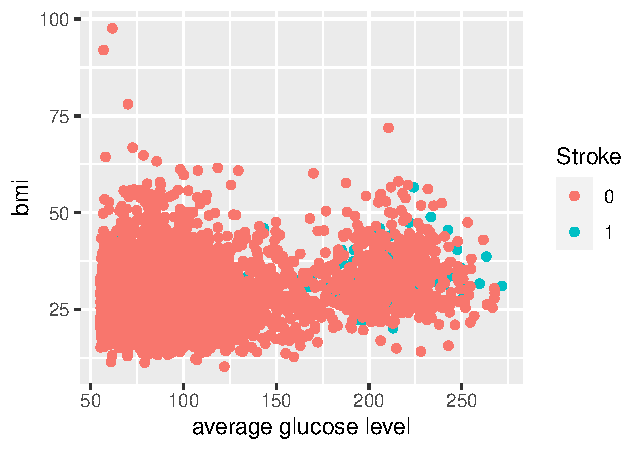
\includegraphics{stat-project-stroke_files/figure-latex/unnamed-chunk-11-1.pdf}

\begin{Shaded}
\begin{Highlighting}[]
\CommentTok{\#boxplot(heart\_disease\textasciitilde{}stroke, xlab=\textquotesingle{}stroke\textquotesingle{} ,ylab = \textquotesingle{}heart\_disease\textquotesingle{})}
\FunctionTok{par}\NormalTok{(}\AttributeTok{mfrow=}\FunctionTok{c}\NormalTok{(}\DecValTok{1}\NormalTok{,}\DecValTok{1}\NormalTok{))}
\end{Highlighting}
\end{Shaded}

Looking at these plots we can see that the incidence of the disease
increases progressively with age and that if we sum also the information
about \texttt{avg\_glucose\_level} we may wonder if diabetic people are
more probable to get a stroke or not. In addition there is no apparent
relation of \texttt{stroke} with \texttt{bmi}.

We now highlight other visual relationship between the variables used
before, thanks to the scatter plots:

\begin{Shaded}
\begin{Highlighting}[]
\FunctionTok{library}\NormalTok{(ggplot2)}
\FunctionTok{ggplot}\NormalTok{(stroke\_data, }\FunctionTok{aes}\NormalTok{(}\AttributeTok{x =}\NormalTok{ avg\_glucose\_level, }\AttributeTok{y =}\NormalTok{ bmi,}\AttributeTok{col =} \FunctionTok{as.factor}\NormalTok{(stroke))) }\SpecialCharTok{+}
  \FunctionTok{labs}\NormalTok{(}\AttributeTok{x =} \StringTok{"average glucose level"}\NormalTok{, }\AttributeTok{y =} \StringTok{"bmi"}\NormalTok{, }\AttributeTok{color =} \StringTok{"Stroke"}\NormalTok{) }\SpecialCharTok{+} \FunctionTok{geom\_point}\NormalTok{()}
\end{Highlighting}
\end{Shaded}

\begin{center}\includegraphics{stat-project-stroke_files/figure-latex/unnamed-chunk-12-1} \end{center}

\begin{Shaded}
\begin{Highlighting}[]
\FunctionTok{ggplot}\NormalTok{(stroke\_data, }\FunctionTok{aes}\NormalTok{(}\AttributeTok{x =}\NormalTok{ avg\_glucose\_level, }\AttributeTok{y =}\NormalTok{ age,}\AttributeTok{col =} \FunctionTok{as.factor}\NormalTok{(stroke))) }\SpecialCharTok{+} 
  \FunctionTok{labs}\NormalTok{(}\AttributeTok{x =} \StringTok{"average glucose level"}\NormalTok{,}\AttributeTok{y =} \StringTok{"age"}\NormalTok{, }\AttributeTok{color =} \StringTok{"Stroke"}\NormalTok{) }\SpecialCharTok{+} \FunctionTok{geom\_point}\NormalTok{()}
\end{Highlighting}
\end{Shaded}

\begin{center}\includegraphics{stat-project-stroke_files/figure-latex/unnamed-chunk-12-2} \end{center}

\begin{Shaded}
\begin{Highlighting}[]
\FunctionTok{ggplot}\NormalTok{(stroke\_data, }\FunctionTok{aes}\NormalTok{(}\AttributeTok{x =}\NormalTok{ bmi, }\AttributeTok{y =}\NormalTok{ age, }\AttributeTok{col =} \FunctionTok{as.factor}\NormalTok{(stroke))) }\SpecialCharTok{+}
  \FunctionTok{labs}\NormalTok{(}\AttributeTok{x =} \StringTok{"bmi"}\NormalTok{, }\AttributeTok{y =} \StringTok{"age"}\NormalTok{, }\AttributeTok{color =} \StringTok{"Stroke"}\NormalTok{) }\SpecialCharTok{+}\FunctionTok{geom\_point}\NormalTok{()}
\end{Highlighting}
\end{Shaded}

\begin{center}\includegraphics{stat-project-stroke_files/figure-latex/unnamed-chunk-12-3} \end{center}

Difficult to read data and give a clear classification/explanation.

Even with high \texttt{avg\_glucose\_level} and \texttt{bmi} it's not so
straightforward to detect the stroke, since they could not be so
strictly related to disease but maybe correlated to other illnesses
linked (or not) to it. In the end it seem to be not so simple to
identify the direct relationship with the stroke while dealing with the
features that we have.

\emph{be related to other disease (which are not correlated with
stroke????) or there are still not enough complications to develop a
stroke. Insomma l'associazione non e` cosi diretta e il problema sembra
essere complicato perche non descrive una chiara classificazione
guardando i punti.}

At this point we can ask some questions:

\begin{itemize}
\tightlist
\item
  Is it possible to prevent ictus?
\item
  Which factors are the most related to it?
\item
  How strong are the relations between the features?
\item
  Are the given variables enough to predict a good accuracy of some
  possible person affected by ictus?
\end{itemize}

We will explore the data trying to answer them.

\hypertarget{modeling}{%
\section{3 Modeling}\label{modeling}}

We will now present some different approaches for the classification of
the data.

\hypertarget{logistic-regression}{%
\subsection{3.1 Logistic Regression}\label{logistic-regression}}

In this part of the predictive analysis we will present three different
type of models, compared to discover the best one that can better
interpret the data.

While going on with the classification using logistic regression we
could meet the following problems: non-linearity of the data,
correlation of error terms, heteroschedasticity, outliers, leverage
point and collinearity.

\hypertarget{full-and-reduced-models}{%
\subsubsection{3.1.1 Full and Reduced
Models}\label{full-and-reduced-models}}

We start with the full model to see if all the features of the dataset
contribute positively/negatively on the prediction of a stroke.

\begin{Shaded}
\begin{Highlighting}[]
\NormalTok{mod.full }\OtherTok{\textless{}{-}} \FunctionTok{glm}\NormalTok{(stroke}\SpecialCharTok{\textasciitilde{}}\NormalTok{., }\AttributeTok{data=}\NormalTok{stroke\_data, }\AttributeTok{family =}\NormalTok{ binomial)}
\FunctionTok{summary}\NormalTok{(mod.full)}
\end{Highlighting}
\end{Shaded}

\begin{verbatim}
## 
## Call:
## glm(formula = stroke ~ ., family = binomial, data = stroke_data)
## 
## Deviance Residuals: 
##     Min       1Q   Median       3Q      Max  
## -1.1823  -0.2947  -0.1524  -0.0744   3.5251  
## 
## Coefficients:
##                              Estimate Std. Error z value Pr(>|z|)    
## (Intercept)                -7.360e+00  1.067e+00  -6.895 5.37e-12 ***
## genderMale                 -1.463e-02  1.544e-01  -0.095 0.924525    
## genderOther                -1.135e+01  2.400e+03  -0.005 0.996225    
## age                         7.348e-02  6.347e-03  11.578  < 2e-16 ***
## hypertension                5.249e-01  1.750e-01   2.999 0.002711 ** 
## heart_disease               3.488e-01  2.072e-01   1.683 0.092381 .  
## ever_marriedYes            -1.152e-01  2.473e-01  -0.466 0.641394    
## work_typeGovt_job          -6.817e-01  1.114e+00  -0.612 0.540660    
## work_typeNever_worked      -1.082e+01  5.090e+02  -0.021 0.983036    
## work_typePrivate           -5.208e-01  1.100e+00  -0.473 0.635943    
## work_typeSelf-employed     -9.459e-01  1.119e+00  -0.845 0.397906    
## Residence_typeUrban         4.514e-03  1.500e-01   0.030 0.975990    
## avg_glucose_level           4.652e-03  1.294e-03   3.595 0.000324 ***
## bmi                         4.062e-03  1.188e-02   0.342 0.732387    
## smoking_statusnever smoked -6.722e-02  1.886e-01  -0.356 0.721556    
## smoking_statussmokes        3.139e-01  2.295e-01   1.368 0.171310    
## smoking_statusUnknown      -2.753e-01  2.471e-01  -1.114 0.265193    
## ---
## Signif. codes:  0 '***' 0.001 '**' 0.01 '*' 0.05 '.' 0.1 ' ' 1
## 
## (Dispersion parameter for binomial family taken to be 1)
## 
##     Null deviance: 1728.4  on 4908  degrees of freedom
## Residual deviance: 1363.2  on 4892  degrees of freedom
## AIC: 1397.2
## 
## Number of Fisher Scoring iterations: 15
\end{verbatim}

Here we see that \texttt{age}, \texttt{avg\_glucose\_level} and
\texttt{hypertension} are the variables most related to \texttt{stroke}.

Let's use the residual plots to get more information about this model
(we use \texttt{type="deviance"} because we have a binary response):

\begin{Shaded}
\begin{Highlighting}[]
\NormalTok{mod.full.resid }\OtherTok{\textless{}{-}} \FunctionTok{residuals}\NormalTok{(mod.full, }\AttributeTok{type=}\StringTok{"deviance"}\NormalTok{) }
\NormalTok{predicted }\OtherTok{\textless{}{-}} \FunctionTok{predict}\NormalTok{(mod.full, }\AttributeTok{type =} \StringTok{"link"}\NormalTok{)}
\FunctionTok{par}\NormalTok{(}\AttributeTok{mfrow=}\FunctionTok{c}\NormalTok{(}\DecValTok{1}\NormalTok{,}\DecValTok{2}\NormalTok{))}
\FunctionTok{plot}\NormalTok{(mod.full.resid}\SpecialCharTok{\textasciitilde{}}\NormalTok{predicted)}
\FunctionTok{abline}\NormalTok{(}\AttributeTok{h=}\DecValTok{0}\NormalTok{, }\AttributeTok{col=}\StringTok{\textquotesingle{}red\textquotesingle{}}\NormalTok{)}
\FunctionTok{qqnorm}\NormalTok{(mod.full.resid)}
\FunctionTok{qqline}\NormalTok{(mod.full.resid, }\AttributeTok{col=}\StringTok{\textquotesingle{}red\textquotesingle{}}\NormalTok{)}
\end{Highlighting}
\end{Shaded}

\includegraphics{stat-project-stroke_files/figure-latex/unnamed-chunk-14-1.pdf}

\begin{Shaded}
\begin{Highlighting}[]
\FunctionTok{par}\NormalTok{(}\AttributeTok{mfrow=}\FunctionTok{c}\NormalTok{(}\DecValTok{1}\NormalTok{,}\DecValTok{1}\NormalTok{))}
\end{Highlighting}
\end{Shaded}

The residual plots are not satisfactory because it is not easy to
interpret them. From the right plot we can see that the data are not
normal.

We now make some test in order to find the best reduced model: we start
from the full model and then remove all the features that have
collinearity between each other,i.e.~\texttt{work\_type},
\texttt{Residence\_type} and \texttt{ever\_married}.

\begin{Shaded}
\begin{Highlighting}[]
\NormalTok{mod.red1 }\OtherTok{\textless{}{-}} \FunctionTok{glm}\NormalTok{(stroke }\SpecialCharTok{\textasciitilde{}}\NormalTok{ age }\SpecialCharTok{+}\NormalTok{ bmi }\SpecialCharTok{+}\NormalTok{ avg\_glucose\_level }\SpecialCharTok{+}\NormalTok{ hypertension }\SpecialCharTok{+} 
\NormalTok{                  smoking\_status }\SpecialCharTok{+}\NormalTok{ gender }\SpecialCharTok{+}\NormalTok{ heart\_disease, }\AttributeTok{family=}\NormalTok{binomial)}
\end{Highlighting}
\end{Shaded}

Also in this case the variables more important are the same of the ones
found in the full moel but also \texttt{heart\_disease} seems to
contribute to the prediction. In this step we try to remove the
\texttt{gender} variable:

\begin{Shaded}
\begin{Highlighting}[]
\NormalTok{mod.red2 }\OtherTok{\textless{}{-}} \FunctionTok{glm}\NormalTok{(stroke }\SpecialCharTok{\textasciitilde{}}\NormalTok{ age }\SpecialCharTok{+}\NormalTok{ bmi }\SpecialCharTok{+}\NormalTok{ avg\_glucose\_level }\SpecialCharTok{+}\NormalTok{ hypertension }\SpecialCharTok{+} 
\NormalTok{                  smoking\_status  }\SpecialCharTok{+}\NormalTok{ heart\_disease, }\AttributeTok{family=}\NormalTok{binomial) }
\FunctionTok{summary}\NormalTok{(mod.red2)}
\end{Highlighting}
\end{Shaded}

The variables left to remove are \texttt{bmi} and
\texttt{smoking\_status}, and we ended up with the final reduced model:
\[\text{mod.red} =\beta_0 + \beta_1\text{age} + \beta_2\text{heart_disease} + \beta_4  \text{avg_glucose_level}+ \beta_5\text{hypertension}\]

\begin{Shaded}
\begin{Highlighting}[]
\NormalTok{mod.red }\OtherTok{\textless{}{-}} \FunctionTok{glm}\NormalTok{(stroke}\SpecialCharTok{\textasciitilde{}}\NormalTok{age }\SpecialCharTok{+}\NormalTok{ heart\_disease }\SpecialCharTok{+}\NormalTok{ avg\_glucose\_level}\SpecialCharTok{+}\NormalTok{ hypertension, }
               \AttributeTok{data=}\NormalTok{stroke\_data, }\AttributeTok{family =}\NormalTok{ binomial)}
\FunctionTok{summary}\NormalTok{(mod.red)}
\end{Highlighting}
\end{Shaded}

\begin{verbatim}
## 
## Call:
## glm(formula = stroke ~ age + heart_disease + avg_glucose_level + 
##     hypertension, family = binomial, data = stroke_data)
## 
## Deviance Residuals: 
##     Min       1Q   Median       3Q      Max  
## -1.0995  -0.2940  -0.1599  -0.0778   3.5885  
## 
## Coefficients:
##                    Estimate Std. Error z value Pr(>|z|)    
## (Intercept)       -7.660740   0.387152 -19.787  < 2e-16 ***
## age                0.067547   0.005571  12.124  < 2e-16 ***
## heart_disease      0.404298   0.203447   1.987 0.046895 *  
## avg_glucose_level  0.004802   0.001255   3.828 0.000129 ***
## hypertension       0.539613   0.173055   3.118 0.001820 ** 
## ---
## Signif. codes:  0 '***' 0.001 '**' 0.01 '*' 0.05 '.' 0.1 ' ' 1
## 
## (Dispersion parameter for binomial family taken to be 1)
## 
##     Null deviance: 1728.4  on 4908  degrees of freedom
## Residual deviance: 1374.6  on 4904  degrees of freedom
## AIC: 1384.6
## 
## Number of Fisher Scoring iterations: 7
\end{verbatim}

For this model we also give a descriptive statistic through the residual
plots:

\begin{Shaded}
\begin{Highlighting}[]
\NormalTok{mod.red.resid }\OtherTok{\textless{}{-}} \FunctionTok{residuals}\NormalTok{(mod.red, }\AttributeTok{type=}\StringTok{"deviance"}\NormalTok{)}
\NormalTok{predicted }\OtherTok{\textless{}{-}} \FunctionTok{predict}\NormalTok{(mod.red, }\AttributeTok{type =} \StringTok{"link"}\NormalTok{)}
\FunctionTok{par}\NormalTok{(}\AttributeTok{mfrow=}\FunctionTok{c}\NormalTok{(}\DecValTok{1}\NormalTok{,}\DecValTok{2}\NormalTok{))}
\FunctionTok{plot}\NormalTok{(mod.red.resid}\SpecialCharTok{\textasciitilde{}}\NormalTok{predicted)}
\FunctionTok{abline}\NormalTok{(}\AttributeTok{h=}\DecValTok{0}\NormalTok{, }\AttributeTok{col=}\StringTok{\textquotesingle{}red\textquotesingle{}}\NormalTok{)}
\FunctionTok{qqnorm}\NormalTok{(mod.red.resid)}
\FunctionTok{qqline}\NormalTok{(mod.red.resid, }\AttributeTok{col=}\StringTok{\textquotesingle{}red\textquotesingle{}}\NormalTok{)}
\end{Highlighting}
\end{Shaded}

\includegraphics{stat-project-stroke_files/figure-latex/unnamed-chunk-18-1.pdf}

\begin{Shaded}
\begin{Highlighting}[]
\FunctionTok{par}\NormalTok{(}\AttributeTok{mfrow=}\FunctionTok{c}\NormalTok{(}\DecValTok{1}\NormalTok{,}\DecValTok{1}\NormalTok{))}
\end{Highlighting}
\end{Shaded}

We can see from the residual vs predicted values the presence of high
non-linearity in the dataset. In the qqplot instead we see that
residuals do no follow a normal distribution.

Positive coefficient estimates ---\textgreater{} positive association.
So, the larger the value, the higher is the estimated probability of
stroke.

Instead in the standard deviance vs predicted we can see that
homoscedasticity does not hold since the line of the standard residual
is not flat, hence even by standardizing the residual we end up having
high variance among residuals.

In the end by looking at the leverage plot, we see the presence of some
sample with high leverage values (bottom right), which could influence
the prediction of the model.

\emph{Buuut I don't know in which range of levarage value is considered
to change a lot the prediction of the model.} Furthermore R does not
show the index of the sample with high leverage, \emph{I guess because a
lot of values could change the prediction.}

Some outliers with high variance are: idx: 119, 183, 246.

In the end, if we compare the results obtained from the full and reduced
models we can say that the reduced seems to make a more accurate
prediction and fits better the data, also the AIC is lower than the one
of the full model. To have a confirmation of this, we use the anova
function, which compare the two models and returns the better between
the two.

\begin{Shaded}
\begin{Highlighting}[]
\FunctionTok{anova}\NormalTok{(mod.full, mod.red, }\AttributeTok{test=}\StringTok{"Chisq"}\NormalTok{)}
\end{Highlighting}
\end{Shaded}

\begin{verbatim}
## Analysis of Deviance Table
## 
## Model 1: stroke ~ gender + age + hypertension + heart_disease + ever_married + 
##     work_type + Residence_type + avg_glucose_level + bmi + smoking_status
## Model 2: stroke ~ age + heart_disease + avg_glucose_level + hypertension
##   Resid. Df Resid. Dev  Df Deviance Pr(>Chi)
## 1      4892     1363.2                      
## 2      4904     1374.7 -12   -11.42   0.4933
\end{verbatim}

As expected from the anova test rejects that the complex model is more
significant than the reduced one, since the p-value is not less than
5\%. Hence the full model does not help with our prediction.

Outliers of the reduced model:

\begin{longtable}[]{@{}lccccccccccc@{}}
\toprule
& gender & age & hypert. & hd & ev\_marr & work\_type & res\_type &
glucose & bmi & smoking & stroke \\
\midrule
\endhead
119 & Female & 38 & 0 & 0 & No & Self-employed & Urban & 82.28 & 24.0 &
formerly smoked & 1 \\
183 & Female & 32 & 0 & 0 & Yes & Private & Rural & 76.13 & 29.9 &
smokes & 1 \\
246 & Female & 14 & 0 & 0 & No & children & Rural & 57.93 & 30.9 &
Unknown & 1 \\
\bottomrule
\end{longtable}

\hypertarget{interaction}{%
\subsubsection{3.1.2 Interaction}\label{interaction}}

In order to see which variables were relevant on our research we tested
various models using the mixed approach: we started by the reduced model
\texttt{mod.red} and then tested some interaction between the
explanatory variables for improving the performance of the model.

We started with \texttt{mod.red}, which had \texttt{stroke} as response
and \texttt{age}, \texttt{avg\_glucose\_level},\texttt{hypertension} and
\texttt{heart\_disease} as predictors. We recall that its AIC was
1384.6.

We then consider the interaction of \texttt{age} with the other
numerical features,
i.e.~\texttt{avg\_glucose\_level},\texttt{hypertension} and
\texttt{heart\_disease}: we find out that only
\texttt{age*heart\_disease} was relevant between the ones tested, with
an AIC = 1384, which was lower than the one of the reduced model
\texttt{mod.red}.

\begin{Shaded}
\begin{Highlighting}[]
\NormalTok{mod1 }\OtherTok{\textless{}{-}} \FunctionTok{glm}\NormalTok{(stroke}\SpecialCharTok{\textasciitilde{}}\NormalTok{age }\SpecialCharTok{+}\NormalTok{ avg\_glucose\_level}\SpecialCharTok{+}\NormalTok{ heart\_disease}\SpecialCharTok{+}\NormalTok{ hypertension }\SpecialCharTok{+}
\NormalTok{               age}\SpecialCharTok{*}\NormalTok{heart\_disease, }\AttributeTok{family=}\NormalTok{binomial)}
\FunctionTok{summary}\NormalTok{(mod1)}
\end{Highlighting}
\end{Shaded}

\begin{verbatim}
## 
## Call:
## glm(formula = stroke ~ age + avg_glucose_level + heart_disease + 
##     hypertension + age * heart_disease, family = binomial)
## 
## Deviance Residuals: 
##     Min       1Q   Median       3Q      Max  
## -0.9897  -0.2980  -0.1557  -0.0737   3.6232  
## 
## Coefficients:
##                    Estimate Std. Error z value Pr(>|z|)    
## (Intercept)       -7.816578   0.407175 -19.197  < 2e-16 ***
## age                0.070133   0.005889  11.908  < 2e-16 ***
## avg_glucose_level  0.004702   0.001253   3.752 0.000176 ***
## heart_disease      2.765299   1.396557   1.980 0.047694 *  
## hypertension       0.536550   0.172602   3.109 0.001880 ** 
## age:heart_disease -0.032872   0.019486  -1.687 0.091604 .  
## ---
## Signif. codes:  0 '***' 0.001 '**' 0.01 '*' 0.05 '.' 0.1 ' ' 1
## 
## (Dispersion parameter for binomial family taken to be 1)
## 
##     Null deviance: 1728.4  on 4908  degrees of freedom
## Residual deviance: 1372.0  on 4903  degrees of freedom
## AIC: 1384
## 
## Number of Fisher Scoring iterations: 7
\end{verbatim}

We went on considering all the interaction of
\texttt{avg\_glucose\_level} with the remaining predictors and find out
that \texttt{avg\_glucose\_level*hypertension} was the best of the
possible interaction but cannot improve the previous model, it had an
AIC of 1385.9.

\begin{Shaded}
\begin{Highlighting}[]
\NormalTok{mod2 }\OtherTok{\textless{}{-}} \FunctionTok{glm}\NormalTok{(stroke}\SpecialCharTok{\textasciitilde{}}\NormalTok{age }\SpecialCharTok{+}\NormalTok{ avg\_glucose\_level}\SpecialCharTok{+}\NormalTok{ heart\_disease}\SpecialCharTok{+}\NormalTok{hypertension }\SpecialCharTok{+}
\NormalTok{              avg\_glucose\_level}\SpecialCharTok{*}\NormalTok{hypertension, }\AttributeTok{family=}\NormalTok{binomial)}
\FunctionTok{summary}\NormalTok{(mod2)}
\end{Highlighting}
\end{Shaded}

In the end it was left the interaction
\texttt{heart\_disease*hypertension} which return an AIC 1384.5 for the
model.

\begin{verbatim}
## 
## Call:
## glm(formula = stroke ~ age + avg_glucose_level + heart_disease + 
##     hypertension + heart_disease * hypertension, family = binomial)
## 
## Deviance Residuals: 
##     Min       1Q   Median       3Q      Max  
## -1.0079  -0.2951  -0.1584  -0.0774   3.5900  
## 
## Coefficients:
##                             Estimate Std. Error z value Pr(>|z|)    
## (Intercept)                -7.657815   0.387787 -19.747  < 2e-16 ***
## age                         0.067108   0.005592  12.001  < 2e-16 ***
## avg_glucose_level           0.004760   0.001256   3.791 0.000150 ***
## heart_disease               0.592399   0.236015   2.510 0.012073 *  
## hypertension                0.660347   0.189663   3.482 0.000498 ***
## heart_disease:hypertension -0.635251   0.444325  -1.430 0.152803    
## ---
## Signif. codes:  0 '***' 0.001 '**' 0.01 '*' 0.05 '.' 0.1 ' ' 1
## 
## (Dispersion parameter for binomial family taken to be 1)
## 
##     Null deviance: 1728.4  on 4908  degrees of freedom
## Residual deviance: 1372.5  on 4903  degrees of freedom
## AIC: 1384.5
## 
## Number of Fisher Scoring iterations: 7
\end{verbatim}

We then tried to see the results of the \texttt{mod.red} without
\texttt{heart\_disease} which was the explanatory variables with higher
p-value, and then we added some interaction terms, starting with the one
with \texttt{age}:

\begin{Shaded}
\begin{Highlighting}[]
\NormalTok{mod4 }\OtherTok{\textless{}{-}} \FunctionTok{glm}\NormalTok{(stroke}\SpecialCharTok{\textasciitilde{}}\NormalTok{age }\SpecialCharTok{+}\NormalTok{ avg\_glucose\_level }\SpecialCharTok{+}\NormalTok{ hypertension }\SpecialCharTok{+} 
\NormalTok{              age}\SpecialCharTok{*}\NormalTok{hypertension, }\AttributeTok{family=}\NormalTok{binomial)}
\FunctionTok{summary}\NormalTok{(mod4)}
\end{Highlighting}
\end{Shaded}

The AIC of this model was 1386.2, higher that the ones seen on the
previous tested models. We go further testing also the interaction add
\texttt{avg\_glucose\_level*hypertension}

\begin{Shaded}
\begin{Highlighting}[]
\NormalTok{mod5 }\OtherTok{\textless{}{-}} \FunctionTok{glm}\NormalTok{(stroke}\SpecialCharTok{\textasciitilde{}}\NormalTok{age }\SpecialCharTok{+}\NormalTok{ avg\_glucose\_level }\SpecialCharTok{+}\NormalTok{ hypertension }\SpecialCharTok{+} 
\NormalTok{              avg\_glucose\_level}\SpecialCharTok{*}\NormalTok{hypertension, }\AttributeTok{family=}\NormalTok{binomial)}
\FunctionTok{summary}\NormalTok{(mod5)}
\end{Highlighting}
\end{Shaded}

It had an AIC = 1387.6. In the end we return on our base model,
\texttt{mod.red} and add the teo best iteractions, i.e.~the two terms
that reduced the AIC term:

\begin{Shaded}
\begin{Highlighting}[]
\NormalTok{mod6 }\OtherTok{\textless{}{-}} \FunctionTok{glm}\NormalTok{(stroke}\SpecialCharTok{\textasciitilde{}}\NormalTok{age }\SpecialCharTok{+}\NormalTok{ avg\_glucose\_level}\SpecialCharTok{+}\NormalTok{ heart\_disease}\SpecialCharTok{+}\NormalTok{ hypertension }\SpecialCharTok{+}
\NormalTok{              age}\SpecialCharTok{*}\NormalTok{heart\_disease }\SpecialCharTok{+}\NormalTok{ heart\_disease}\SpecialCharTok{*}\NormalTok{hypertension, }\AttributeTok{family=}\NormalTok{binomial)}
\FunctionTok{summary}\NormalTok{(mod6)}
\end{Highlighting}
\end{Shaded}

It has AIC = 1384.2 but the interactions had a p-value greater than 0.1
and it didn't seem to represent our data properly. At the end of all we
promote \texttt{mod1} as the model which better fits our data.

Let's now see some relevant information, such as outliers on the
\texttt{mod1}:

\begin{longtable}[]{@{}lccccccccccc@{}}
\toprule
& gender & age & hypert. & hd & ev\_marr & work\_type & res\_type &
glucose & bmi & smoking & stroke \\
\midrule
\endhead
207 & Female & 81 & 0 & 0 & Yes & Private & Rural & 80.13 & 23.4 & never
smoked & 1 \\
150 & Female & 70 & 0 & 1 & Yes & Private & Rural & 239.07 & 26.1 &
never smoked & 1 \\
100 & Female & 69 & 0 & 0 & Yes & Govt\_job & Urban & 82.81 & 28.0 &
never smoked & 1 \\
\bottomrule
\end{longtable}

but also leverage point and collinearity:

\begin{Shaded}
\begin{Highlighting}[]
\FunctionTok{plot}\NormalTok{(mod1)}
\end{Highlighting}
\end{Shaded}

\includegraphics{stat-project-stroke_files/figure-latex/unnamed-chunk-28-1.pdf}
\includegraphics{stat-project-stroke_files/figure-latex/unnamed-chunk-28-2.pdf}
\includegraphics{stat-project-stroke_files/figure-latex/unnamed-chunk-28-3.pdf}
\includegraphics{stat-project-stroke_files/figure-latex/unnamed-chunk-28-4.pdf}

\hypertarget{polynomial-models}{%
\subsubsection{3.1.3 Polynomial models}\label{polynomial-models}}

We tried to use a polynomial model starting from the reduced model
\texttt{mod.red} with also \texttt{bmi} as predictors. Then we
contribute with the square of \texttt{bmi}, \texttt{avg\_glucose\_level}
and then both for the \texttt{mod.poly1},\texttt{mod.poly2} and
\texttt{mod.poly3} respectively.

\begin{Shaded}
\begin{Highlighting}[]
\NormalTok{mod.poly1 }\OtherTok{\textless{}{-}} \FunctionTok{glm}\NormalTok{(stroke}\SpecialCharTok{\textasciitilde{}}\NormalTok{age }\SpecialCharTok{+}\NormalTok{ heart\_disease }\SpecialCharTok{+}\NormalTok{ avg\_glucose\_level}\SpecialCharTok{+}\NormalTok{ hypertension}\SpecialCharTok{+}\NormalTok{bmi}\SpecialCharTok{+}
                       \FunctionTok{I}\NormalTok{(bmi}\SpecialCharTok{\^{}}\DecValTok{2}\NormalTok{), }\AttributeTok{family =}\NormalTok{ binomial)}
\FunctionTok{summary}\NormalTok{(mod.poly1)}
\NormalTok{mod.poly2 }\OtherTok{\textless{}{-}} \FunctionTok{glm}\NormalTok{(stroke}\SpecialCharTok{\textasciitilde{}}\NormalTok{age }\SpecialCharTok{+}\NormalTok{ heart\_disease }\SpecialCharTok{+}\NormalTok{ avg\_glucose\_level}\SpecialCharTok{+}\NormalTok{ hypertension}\SpecialCharTok{+}\NormalTok{bmi}\SpecialCharTok{+}
                     \SpecialCharTok{+} \FunctionTok{I}\NormalTok{(avg\_glucose\_level}\SpecialCharTok{\^{}}\DecValTok{2}\NormalTok{), }\AttributeTok{family =}\NormalTok{ binomial)}
\FunctionTok{summary}\NormalTok{(mod.poly2)}
\NormalTok{mod.poly3 }\OtherTok{\textless{}{-}} \FunctionTok{glm}\NormalTok{(stroke}\SpecialCharTok{\textasciitilde{}}\NormalTok{age }\SpecialCharTok{+}\NormalTok{ heart\_disease }\SpecialCharTok{+}\NormalTok{ avg\_glucose\_level}\SpecialCharTok{+}\NormalTok{ hypertension}\SpecialCharTok{+}\NormalTok{bmi}\SpecialCharTok{+}
                      \FunctionTok{I}\NormalTok{(bmi}\SpecialCharTok{\^{}}\DecValTok{2}\NormalTok{) }\SpecialCharTok{+} \FunctionTok{I}\NormalTok{(avg\_glucose\_level}\SpecialCharTok{\^{}}\DecValTok{2}\NormalTok{), }\AttributeTok{family =}\NormalTok{ binomial)}
\FunctionTok{summary}\NormalTok{(mod.poly3)}
\end{Highlighting}
\end{Shaded}

At the end of the tests nothing interesting appeared with polynomial
models. There were no improvement in the results.

\hypertarget{lda}{%
\subsection{3.2 LDA}\label{lda}}

Assumption: samples are normally distributed and have same variance in
every class =\textgreater{} strong assumption.

\begin{Shaded}
\begin{Highlighting}[]
\FunctionTok{library}\NormalTok{(MASS)}
\NormalTok{lda.fit }\OtherTok{\textless{}{-}} \FunctionTok{lda}\NormalTok{(stroke}\SpecialCharTok{\textasciitilde{}}\NormalTok{age}\SpecialCharTok{+}\NormalTok{bmi}\SpecialCharTok{+}\NormalTok{avg\_glucose\_level}\SpecialCharTok{+}\NormalTok{hypertension}\SpecialCharTok{+}\NormalTok{work\_type}\SpecialCharTok{+}\NormalTok{gender}
               \SpecialCharTok{+}\NormalTok{smoking\_status}\SpecialCharTok{+}\NormalTok{ever\_married}\SpecialCharTok{+}\NormalTok{Residence\_type }\SpecialCharTok{+}\NormalTok{ heart\_disease)}
\NormalTok{lda.pred }\OtherTok{\textless{}{-}} \FunctionTok{predict}\NormalTok{(lda.fit)}
\FunctionTok{table}\NormalTok{(lda.pred}\SpecialCharTok{$}\NormalTok{class, stroke)}
\end{Highlighting}
\end{Shaded}

\begin{verbatim}
##    stroke
##        0    1
##   0 4646  186
##   1   54   23
\end{verbatim}

\begin{Shaded}
\begin{Highlighting}[]
\NormalTok{lda.pred.stroke }\OtherTok{\textless{}{-}}\NormalTok{ lda.pred}\SpecialCharTok{$}\NormalTok{posterior[, }\DecValTok{2}\NormalTok{]}
\end{Highlighting}
\end{Shaded}

\hypertarget{qda}{%
\subsection{3.3 QDA}\label{qda}}

Assumption: sample are normally distributed BUT NOT SAME variance among
classes.

\begin{Shaded}
\begin{Highlighting}[]
\NormalTok{qda.fit }\OtherTok{\textless{}{-}} \FunctionTok{qda}\NormalTok{(stroke}\SpecialCharTok{\textasciitilde{}}\NormalTok{age}\SpecialCharTok{+}\NormalTok{bmi}\SpecialCharTok{+}\NormalTok{avg\_glucose\_level}\SpecialCharTok{+}\NormalTok{hypertension}\SpecialCharTok{+}\NormalTok{heart\_disease}\SpecialCharTok{+}\NormalTok{smoking\_status, }\AttributeTok{data =}\NormalTok{ stroke\_data)}
\CommentTok{\# ERROR rank deficiency, i.e. some variables }
\CommentTok{\# are collinear and one or more covariance matrices cannot be inverted to obtain the estimates in group 1 (Controls)!}
\NormalTok{qda.pred }\OtherTok{\textless{}{-}} \FunctionTok{predict}\NormalTok{(qda.fit, stroke\_data)}
\NormalTok{qda.pred.stroke }\OtherTok{\textless{}{-}}\NormalTok{ qda.pred}\SpecialCharTok{$}\NormalTok{posterior[, }\DecValTok{2}\NormalTok{]}
\FunctionTok{table}\NormalTok{(qda.pred}\SpecialCharTok{$}\NormalTok{class, stroke)}
\end{Highlighting}
\end{Shaded}

\begin{verbatim}
##    stroke
##        0    1
##   0 4260  123
##   1  440   86
\end{verbatim}

\hypertarget{predictions}{%
\section{4 Predictions}\label{predictions}}

In order to split the dataset into validation, training and test sets we
recall that the amount of data that we have is of 4909, so we decided to
keep approximately the 75\% of the data for the training phase: 3682
people of which 3562 are the ones which hadn't the stroke, while 120 had
it. We didn't use the cross-validation because it was difficult to split
tha data and bla bla.

\textbf{CODICE CORRETTO}

\hypertarget{roc-and-precision-recall-curves}{%
\subsection{4.1 ROC and PRECISION-RECALL
Curves}\label{roc-and-precision-recall-curves}}

We introduced an hand-written function to make usefull plot because
Allora ieri guardando i plot della ROC curve io e francesca c'eravamo
posti due domande sui risultati. Siccome siamo in un problema medico di
predizione di ictus di un paziente oppure no, alla fine la ROC curve non
e\texttt{molto\ d\textquotesingle{}aiuto\ perche\ massimizza\ i\ true\ positive\ con\ i\ true\ predicted.\ \ Questo\ significa\ che\ possibilmenete\ gli\ errori\ di\ false\ negativo\ possono\ incrementare.\ In\ ambito\ del\ nostro\ problema\ e\ in\ generale\ in\ ambito\ medico\ se\ il\ nostro\ modello\ predice\ una\ persona\ senza\ ictus\ quando\ invece\ lo\ presenta,\ eh\ \ questa\ e}
un errore piu grave rispetto a un false positive. Noi vorremmo invece
che il false negative sia basso e quindi considerato. Insomma significa
che dobbiamo usare la Precision Recall curve.

\begin{Shaded}
\begin{Highlighting}[]
\FunctionTok{library}\NormalTok{(pROC)}
\end{Highlighting}
\end{Shaded}

\begin{verbatim}
## Type 'citation("pROC")' for a citation.
\end{verbatim}

\begin{verbatim}
## 
## Caricamento pacchetto: 'pROC'
\end{verbatim}

\begin{verbatim}
## I seguenti oggetti sono mascherati da 'package:stats':
## 
##     cov, smooth, var
\end{verbatim}

\begin{Shaded}
\begin{Highlighting}[]
\FunctionTok{library}\NormalTok{(ROCR)}
\NormalTok{get.roc.recall.values }\OtherTok{\textless{}{-}} \ControlFlowTok{function}\NormalTok{(pred\_models, true\_value) \{}
\NormalTok{  result }\OtherTok{\textless{}{-}} \FunctionTok{data.frame}\NormalTok{(}\AttributeTok{Threshold1=}\FunctionTok{double}\NormalTok{(), }\AttributeTok{Specificity=}\FunctionTok{double}\NormalTok{(), }\AttributeTok{Sensitivity=}\FunctionTok{double}\NormalTok{(),}
                       \AttributeTok{Threshold2=}\FunctionTok{double}\NormalTok{(), }\AttributeTok{Recall=}\FunctionTok{double}\NormalTok{(), }\AttributeTok{Precision=}\FunctionTok{double}\NormalTok{())}
\NormalTok{  n\_models }\OtherTok{=} \FunctionTok{length}\NormalTok{(}\FunctionTok{list}\NormalTok{(mod.red.probs,lda.pred.stroke, qda.pred.stroke))}
  \FunctionTok{par}\NormalTok{(}\AttributeTok{mfrow=}\FunctionTok{c}\NormalTok{(n\_models, }\DecValTok{2}\NormalTok{))}
  \ControlFlowTok{for}\NormalTok{ (pred }\ControlFlowTok{in}\NormalTok{ pred\_models) \{}
\NormalTok{    roc.res }\OtherTok{\textless{}{-}} \FunctionTok{roc}\NormalTok{(true\_value, pred, }\AttributeTok{levels=}\FunctionTok{c}\NormalTok{(}\StringTok{"0"}\NormalTok{, }\StringTok{"1"}\NormalTok{))}
    \FunctionTok{plot}\NormalTok{(roc.res, }\AttributeTok{print.auc=}\ConstantTok{TRUE}\NormalTok{, }\AttributeTok{legacy.axes=}\ConstantTok{TRUE}\NormalTok{, }\AttributeTok{xlab=}\StringTok{"False positive rate"}\NormalTok{, }
         \AttributeTok{ylab=}\StringTok{"True positive rate"}\NormalTok{)}
    
\NormalTok{    tmp.res  }\OtherTok{\textless{}{-}} \FunctionTok{coords}\NormalTok{(roc.res, }\StringTok{"best"}\NormalTok{)}
\NormalTok{    pred.rec }\OtherTok{=} \FunctionTok{prediction}\NormalTok{(mod.red.probs, true\_value)}
\NormalTok{    perf }\OtherTok{=} \FunctionTok{performance}\NormalTok{(pred.rec, }\StringTok{"prec"}\NormalTok{, }\StringTok{"rec"}\NormalTok{)}
    \FunctionTok{plot}\NormalTok{(perf)}
\NormalTok{    pr\_cutoffs }\OtherTok{\textless{}{-}} \FunctionTok{data.frame}\NormalTok{(}\AttributeTok{cutrecall=}\NormalTok{perf}\SpecialCharTok{@}\NormalTok{alpha.values[[}\DecValTok{1}\NormalTok{]], }\AttributeTok{recall=}\NormalTok{perf}\SpecialCharTok{@}\NormalTok{x.values[[}\DecValTok{1}\NormalTok{]], }
                             \AttributeTok{precision=}\NormalTok{perf}\SpecialCharTok{@}\NormalTok{y.values[[}\DecValTok{1}\NormalTok{]])}
\NormalTok{    best\_recall }\OtherTok{\textless{}{-}}\NormalTok{ pr\_cutoffs[}\FunctionTok{which.min}\NormalTok{(pr\_cutoffs}\SpecialCharTok{$}\NormalTok{recall }\SpecialCharTok{+}\NormalTok{ pr\_cutoffs}\SpecialCharTok{$}\NormalTok{precision), ]}
    
\NormalTok{    result[}\FunctionTok{nrow}\NormalTok{(result) }\SpecialCharTok{+} \DecValTok{1}\NormalTok{,] }\OtherTok{=} \FunctionTok{c}\NormalTok{(tmp.res[}\DecValTok{1}\NormalTok{, }\DecValTok{1}\NormalTok{], tmp.res[}\DecValTok{1}\NormalTok{, }\DecValTok{2}\NormalTok{], tmp.res[}\DecValTok{1}\NormalTok{, }\DecValTok{3}\NormalTok{], }
\NormalTok{                                  best\_recall[}\DecValTok{1}\NormalTok{, }\DecValTok{1}\NormalTok{], best\_recall[}\DecValTok{1}\NormalTok{, }\DecValTok{2}\NormalTok{], best\_recall[}\DecValTok{1}\NormalTok{, }\DecValTok{3}\NormalTok{])}
\NormalTok{  \}}
  \FunctionTok{par}\NormalTok{(}\AttributeTok{mfrow=}\FunctionTok{c}\NormalTok{(}\DecValTok{1}\NormalTok{, }\DecValTok{1}\NormalTok{))}
  \FunctionTok{return}\NormalTok{(result)}
\NormalTok{\}}
\NormalTok{mod.red }\OtherTok{\textless{}{-}} \FunctionTok{glm}\NormalTok{(stroke}\SpecialCharTok{\textasciitilde{}}\NormalTok{age }\SpecialCharTok{+}\NormalTok{ avg\_glucose\_level }\SpecialCharTok{+}\NormalTok{ hypertension }\SpecialCharTok{+}\NormalTok{ bmi, }\AttributeTok{data=}\NormalTok{stroke\_data, }
               \AttributeTok{family =}\NormalTok{ binomial)}
\FunctionTok{summary}\NormalTok{(mod.red)}
\end{Highlighting}
\end{Shaded}

\begin{verbatim}
## 
## Call:
## glm(formula = stroke ~ age + avg_glucose_level + hypertension + 
##     bmi, family = binomial, data = stroke_data)
## 
## Deviance Residuals: 
##     Min       1Q   Median       3Q      Max  
## -1.0265  -0.2986  -0.1600  -0.0755   3.6075  
## 
## Coefficients:
##                    Estimate Std. Error z value Pr(>|z|)    
## (Intercept)       -7.852291   0.541579 -14.499  < 2e-16 ***
## age                0.069793   0.005593  12.479  < 2e-16 ***
## avg_glucose_level  0.004984   0.001276   3.905 9.41e-05 ***
## hypertension       0.543399   0.173304   3.136  0.00172 ** 
## bmi                0.002621   0.011598   0.226  0.82121    
## ---
## Signif. codes:  0 '***' 0.001 '**' 0.01 '*' 0.05 '.' 0.1 ' ' 1
## 
## (Dispersion parameter for binomial family taken to be 1)
## 
##     Null deviance: 1728.4  on 4908  degrees of freedom
## Residual deviance: 1378.4  on 4904  degrees of freedom
## AIC: 1388.4
## 
## Number of Fisher Scoring iterations: 7
\end{verbatim}

\begin{Shaded}
\begin{Highlighting}[]
\NormalTok{mod.red.probs }\OtherTok{\textless{}{-}} \FunctionTok{predict}\NormalTok{(mod.red,}\AttributeTok{type=}\StringTok{"response"}\NormalTok{)}
\end{Highlighting}
\end{Shaded}

\hypertarget{training-set}{%
\subsection{4.2 Training Set}\label{training-set}}

Insertion of the no-stroke people into the training set:

\begin{Shaded}
\begin{Highlighting}[]
\NormalTok{no.strokes.data }\OtherTok{\textless{}{-}}\NormalTok{ stroke\_data[stroke }\SpecialCharTok{==} \DecValTok{0}\NormalTok{, ]}
\NormalTok{rnd.idx.no.strokes }\OtherTok{\textless{}{-}} \FunctionTok{sample}\NormalTok{(}\FunctionTok{c}\NormalTok{(}\DecValTok{1}\SpecialCharTok{:}\FunctionTok{dim}\NormalTok{(no.strokes.data)[}\DecValTok{1}\NormalTok{]))}
\end{Highlighting}
\end{Shaded}

Insertion of the stroke people into the training set:

\begin{Shaded}
\begin{Highlighting}[]
\NormalTok{yes.strokes.data }\OtherTok{\textless{}{-}}\NormalTok{ stroke\_data[stroke }\SpecialCharTok{==} \DecValTok{1}\NormalTok{, ]}
\NormalTok{rnd.idx.yes.strokes }\OtherTok{\textless{}{-}} \FunctionTok{sample}\NormalTok{(}\FunctionTok{c}\NormalTok{(}\DecValTok{1}\SpecialCharTok{:}\FunctionTok{dim}\NormalTok{(yes.strokes.data)[}\DecValTok{1}\NormalTok{]))}
\end{Highlighting}
\end{Shaded}

We mix together the two parts and we use the \texttt{shuffle} function
because the strokes are added in the last positions

\begin{Shaded}
\begin{Highlighting}[]
\NormalTok{training.set }\OtherTok{\textless{}{-}}\NormalTok{ no.strokes.data[rnd.idx.no.strokes[}\DecValTok{1}\SpecialCharTok{:}\DecValTok{3562}\NormalTok{], ]}
\NormalTok{training.set }\OtherTok{\textless{}{-}} \FunctionTok{rbind}\NormalTok{(training.set, yes.strokes.data[rnd.idx.yes.strokes[}\DecValTok{1}\SpecialCharTok{:}\DecValTok{120}\NormalTok{], ])}
\NormalTok{shuffle }\OtherTok{\textless{}{-}} \FunctionTok{sample}\NormalTok{(}\FunctionTok{nrow}\NormalTok{(training.set))}
\NormalTok{training.set }\OtherTok{\textless{}{-}}\NormalTok{ training.set[shuffle, ]}
\end{Highlighting}
\end{Shaded}

\hypertarget{validation-set}{%
\subsection{4.3 Validation Set}\label{validation-set}}

We mix shuffle together the remaining samples into forming the
validation set.

\begin{Shaded}
\begin{Highlighting}[]
\NormalTok{val.set }\OtherTok{\textless{}{-}}\NormalTok{ no.strokes.data[rnd.idx.no.strokes[}\DecValTok{3563}\SpecialCharTok{:}\DecValTok{4700}\NormalTok{], ]}
\NormalTok{val.set }\OtherTok{\textless{}{-}} \FunctionTok{rbind}\NormalTok{(val.set, yes.strokes.data[rnd.idx.yes.strokes[}\DecValTok{121}\SpecialCharTok{:}\DecValTok{209}\NormalTok{], ])}
\NormalTok{shuffle }\OtherTok{\textless{}{-}} \FunctionTok{sample}\NormalTok{(}\FunctionTok{nrow}\NormalTok{(val.set)) }
\NormalTok{val.set }\OtherTok{\textless{}{-}}\NormalTok{ val.set[shuffle, ]}
\end{Highlighting}
\end{Shaded}

\hypertarget{conclusions}{%
\section{5 Conclusions}\label{conclusions}}

Si stima che la percentuale di persone che possono avere un ictus andrà
via via crescendo dal momento che l'età media della popolazione è in
costante crescita.

\end{document}
